\documentclass[10pt,fleqn]{article} % Default font size and left-justified equations
\usepackage[%
    pdftitle={Résolutions de problèmes de statique : PFS 3D},
    pdfauthor={Xavier Pessoles}]{hyperref}

\input{style/new_style}
\input{style/macros_SII}
\usepackage{multicol}
\usepackage{siunitx}
%\usepackage{picins}
\fichetrue
%\fichefalse

\proftrue
\proffalse

\tdtrue
%\tdfalse

\courstrue
\coursfalse

\newif\ifnormal
\normaltrue
%\normalfalse

\newif\ifdifficile
\difficilefalse
%\difficiletrue

\newif\iftdifficile
\tdifficilefalse
%\tdifficiletrue

% -------------------------------------
% Déclaration des titres
% -------------------------------------

\def\classe{\textsf{PSI$\star$ -- MP}}
\def\xxnumpartie{Cycle 06}
\def\xxpartie{Modéliser le comportement des systèmes mécaniques dans le but d'établir une loi de comportement ou de déterminer des actions mécaniques en utilisant les méthodes énergétiques}

\def\xxnumchapitre{Chapitre 1 \vspace{.2cm}}
\def\xxchapitre{\hspace{.12cm} Approche énergétique}

\def\discipline{Sciences \\Industrielles de \\ l'Ingénieur}
\def\xxtete{Sciences Industrielles de l'Ingénieur}

\def\xxposongletx{2}
\def\xxposonglettext{1.45}
\def\xxposonglety{19}%16

\def\xxonglet{\textsf{Cycle 06}}

\def\xxactivite{TD 03}
\def\xxauteur{\textsl{Xavier Pessoles}}


\def\xxtitreexo{Récupération d’énergie au freinage sur véhicules électriques \ifnormal $\star$ \else \fi \iftdifficile $\star\star\star$ \else \fi }
\def\xxsourceexo{\hspace{.2cm} \footnotesize{Concours Centrale Supelec MP -- 2012}}

\def\xxcompetences{%
\textsl{%
\textbf{Savoirs et compétences :}\\
}}

\def\xxfigures{
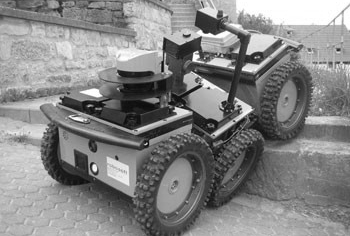
\includegraphics[width=.75\textwidth]{images/fig_00}
}%figues de la page de garde
\def\xxpied{%
Cycle 06 -- Modélisation mécanique -- Énergétique\\% afin de valider leurs performances.\\
Chapitre 1 -- \xxactivite%
}


\setcounter{secnumdepth}{5}
%---------------------------------------------------------------------------


\begin{document}
%\chapterimage{png/Fond_Cin}
\input{style/new_pagegarde}
\vspace{4.5cm}
\pagestyle{fancy}
\thispagestyle{plain}


\def\columnseprulecolor{\color{ocre}}
\setlength{\columnseprule}{0.4pt} 

\ifprof
%\begin{multicols}{2}
\else
\begin{multicols}{2}
\fi

\section*{Mise en situation}
\ifprof
\else
Pour réduire l’empreinte carbone du secteur transport des particuliers, plusieurs constructeurs automobiles
développent des véhicules électriques avec des systèmes de récupération d’énergie au freinage. %Le principe de
%récupération d’énergie est identique chez tous les constructeurs mais la réalisation et les algorithmes diffèrent
%quelque peu. Le support utilisé comme illustration de ce principe innovant est la Renault « Fluence Zéro
%Émission » commercialisée courant 2012 en Europe. Afin de respecter la confidentialité du développement de ce
%véhicule, les données ont été modifiées pour les besoins de ce sujet et les cas d’usage étudiés sont limitatifs.


\begin{center}
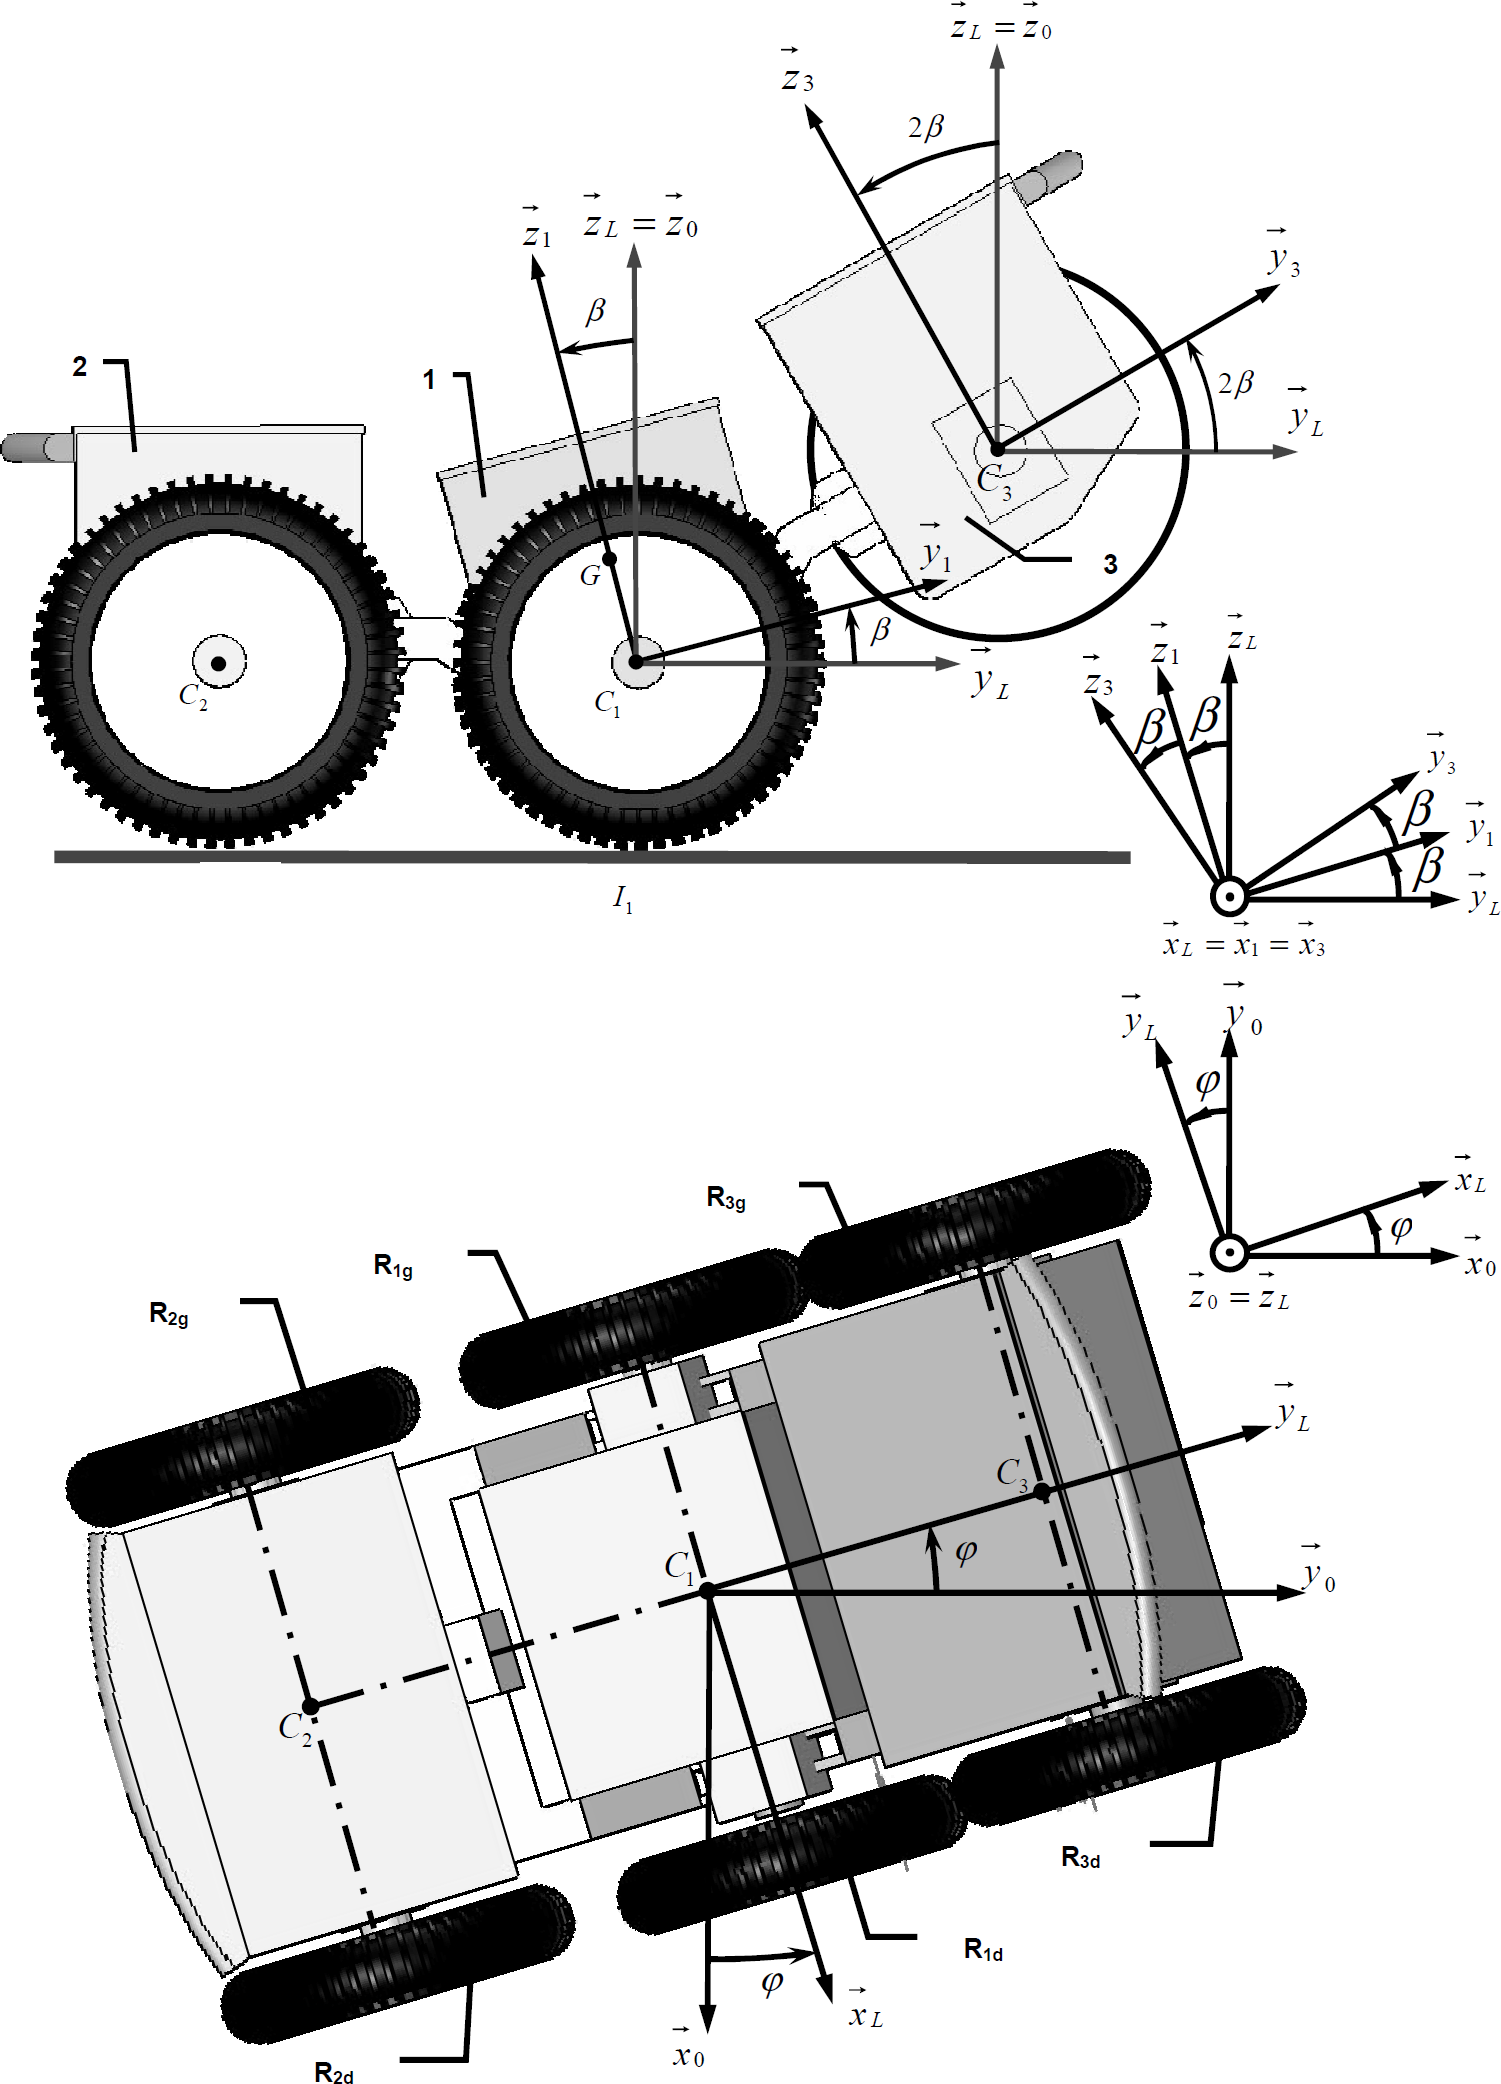
\includegraphics[width=\linewidth]{images/fig_01}
%\textit{}
\end{center}

\section*{Pertinence de la récupération d'énergie au freinage}
\begin{obj}
Valider la pertinence d’un système de récupération d’énergie au freinage et mettre en évidence les
limites d’un freinage purement électrique.
\end{obj}

\section*{Analyse fonctionnelle externe}

Afin de minimiser la consommation électrique des véhicules électriques, une solution consiste à récupérer l’énergie
cinétique et/ou potentielle du véhicule lors des phases de freinage. Pour cela, on exploite la réversibilité de la
chaîne d’énergie électrique en faisant fonctionner l’actionneur électrique de la chaîne de transmission en mode
générateur.


On appelle séquence urbaine type, un trajet entre deux feux tricolores, en ligne droite, sur une route horizontale
et composé :
\begin{itemize}
\item d’une phase d’accélération de 0 à $\SI{50}{km.h^{-1}}$ (durée $t_1 - t_0 = t_a$);
\item d’un parcours de \SI{500}{m} à une vitesse constante de $V_0 =\SI{50}{km.h^{-1}}$ (durée $t_2- t_1$);
\item puis d’une phase de décélération (durée $t_3 -t_2 =t_f$ ) avec arrêt au feu à l’instant $t_3$ en respectant la situation
de freinage nominal évoquée précédemment.
\end{itemize}

La décélération commandée par la levée du pied de la pédale d’accélérateur correspond
au « frein moteur » d’un véhicule thermique. Pour des raisons de confort
et d’habitude de conduite, elle est choisie proche de \SI{2}{m.s^{-2}}. %Cette valeur est
%légèrement supérieure à celle obtenue par le frein moteur d’un véhicule thermique.
%De plus, cette décélération a l’avantage d’être très reproductible, contrairement à
%celle d’un véhicule thermique qui est fonction notamment de la vitesse engagée.
%Sur un véhicule électrique, le compte-tours est remplacé par un compteur dédié
%aux informations relatives à l’autonomie, en particulier le niveau de charge de la
%batterie.


\subparagraph{}\textit{Indiquer trois raisons incitant les usagers des véhicules électriques à décélérer sans utiliser la pédale de frein, par rapport aux habitudes de conduite d’un véhicule thermique.}
\ifprof
\begin{corrige}
\end{corrige}
\else
\fi

\subsection*{Étude de la séquence urbaine type}

On adopte un modèle ramené dans le plan $\left(\vect{x},\vect{y}\right)$, dans la mesure où l’on considérera que le véhicule se déplace en ligne droite horizontale.

\begin{center}
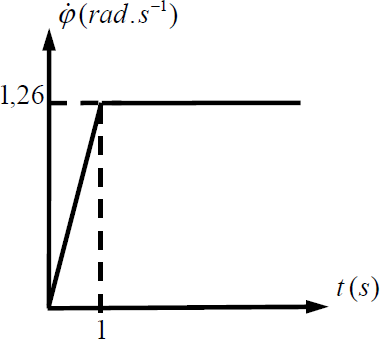
\includegraphics[width=\linewidth]{images/fig_02}

%\textit{Modèle volumique 3D}
\end{center}

On note :
\begin{itemize}
\item $\vect{V}_{\text{Vehicule/sol}} = -V_h(t)\vect{x}$ la vitesse du véhicule par rapport au sol;
\item $\vect{\gamma}_{\text{Vehicule/sol}} = -\gamma(t)\vect{x}$ la vitesse du véhicule par rapport au sol.
\end{itemize}

\subparagraph{}\textit{Dans le cas d'un freinage nominal, $\gamma(t)=\gamma_n=-2\SI{2}{m.s^{-2}}$ déterminer la distance parcourue en partant d'une vitesse initiale $V_0=\SI{50}{km.h^{-1}}$. Conclure au regard des critères du cahier des charges.}
\ifprof
\begin{corrige}
\end{corrige}
\else
\fi


Pour simplifier, on considère que la phase d’accélération de 0 à \SI{50}{km.h^{-1}} se fait avec l’accélération $\gamma(t)=-\gamma_n = \SI{2}{m.s^{-2}}$. 


\subparagraph{}\textit{Tracer l’évolution temporelle de la vitesse $V_h(t)$ du véhicule par rapport au sol en fonction du temps sur la séquence urbaine type et définir son expression en fonction de $\gamma_n$, $V_0$ et $t_2$ sur chaque intervalle de temps $[t_0, t_1]$, $[t_1, t_2]$ et $[t_2, t_3]$. Donner les valeurs numériques des durées $t_1 -t_0 = t_a$, $t_2 - t_1$ et $t_3 - t_2 = t_f$ .}
\ifprof
\begin{corrige}
\end{corrige}
\else
\fi

\subsection*{Pertinence de la récupération d’énergie au freinage}

\subsubsection*{Paramétrage des sources dissipatrices d’énergie}
Pour valider la pertinence d’un système de récupération d’énergie au freinage, on se propose d’évaluer la quantité
d’énergie fournie par la batterie puis restituée à la batterie au cours d’une séquence urbaine type.
Le véhicule étudié a une masse $M = \SI{1600}{kg}$. La chaîne d’énergie est constituée d’une électronique de puissance,
d’une machine électrique et d’une transmission mécanique.

La puissance perdue par la chaîne d’énergie utilisée en mode traction du véhicule s’exprime sous la forme
$P_{\text{perdue directe}} = -(1-\eta)P_{\text {élec}}$ où $P_{\text{élec}}$ ($P_{\text{élec}}>0$) est la puissance électrique fournie par la batterie et $\eta$ le facteur de perte avec $\eta = 0,7$.
Pour cette même chaîne d’énergie utilisée en mode récupération de l’énergie au freinage (tout électrique), la
puissance perdue s’exprime sous la forme $P_{\text{perdue inverse}}= (1/\eta - 1)P_{\text{élec}}$
où $P_{\text{élec}}$ ($P_{\text{élec}}<0$) est la puissance électrique récupérée par la batterie.

On suppose par ailleurs qu’un effort résistant de type visqueux, correspondant d’une part aux frottements
aérodynamiques, et d’autre part à la résistance au roulement, s’oppose à l’avancement du véhicule et que sa
norme s’exprime sous la forme $fV_h(t)$, avec $f = \SI{16}{N.s.m^{-1}}$.

\subsubsection*{Énergie fournie par la batterie pendant la phase d’accélération}


\subparagraph{}\textit{En précisant clairement le théorème utilisé et les hypothèses considérées, déterminer l’expression de la puissance fournie par la batterie, $P_{\text{élec}}(t)$, pour accélérer le véhicule de 0 à $V_0 = \SI{50}{km.h^{-1}}$ en fonction de $M$, $f$, $\eta$, $V_h(t)$ et $\gamma_n$.}
\ifprof
\begin{corrige}
\end{corrige}
\else
\fi


\subparagraph{}\textit{En déduire l’expression de l’énergie fournie par la batterie pendant cette phase d’accélération en fonction de $M$, $f$, $\eta$, $V_0$ et $\gamma_n$. Faire l’application numérique.}
\ifprof
\begin{corrige}
\end{corrige}
\else
\fi

\subsubsection*{Énergie fournie par la batterie pendant la phase à vitesse constante}


\subparagraph{}\textit{En utilisant la même démarche, déterminer l’énergie fournie par la batterie pendant la phase à vitesse constante $V_0 = \SI{50}{km.h^{-1}}$.}
\ifprof
\begin{corrige}
\end{corrige}
\else
\fi



\subsubsection*{Énergie récupérable par la batterie pendant la phase de freinage}

Pour le modèle avec effort résistant de type visqueux, l’énergie récupérée dans la batterie si on exploite la
réversibilité de la chaîne de transmission lors d’un freinage nominal, est égale à $E_{50-0\text{élec}} = -\SI{103}{kJ}$.

Pour un modèle sans effort résistant de type visqueux, l’énergie récupérée dans la batterie, si on exploite la
réversibilité de la chaîne de transmission lors d’un freinage nominal, est égale à $E'_{50-0\text{élec}} = -\SI{108}{kJ}$.

\subparagraph{}\textit{Comparer ces deux résultats et conclure.}
\ifprof
\begin{corrige}
\end{corrige}
\else
\fi

\subsubsection*{Conclusion}

\subparagraph{}\textit{En déduire alors la pertinence du système de récupération d’énergie électrique.}
\ifprof
\begin{corrige}
\end{corrige}
\else
\fi


\subsection*{Limites du freinage électrique}
On note :
\begin{itemize}
\item $\vect{C}_F = -C_F (t)\vect{z}$, le couple de freinage uniquement exercé sur la paire de roues avant du véhicule. La chaîne d’énergie du véhicule étudié entraîne uniquement l’essieu avant. En phase de freinage $C_F (t) > 0$;
\item $R_r$, le rayon des quatre roues, $R_r = \SI{0,3}{m}$.
\end{itemize}
Hypothèses :
\begin{itemize}
\item on négligera l’inertie des roues pour cette pré-étude ;
\item on suppose que les roues ne glissent pas par rapport au sol ;
\item l’effort résistant de type visqueux sera désormais négligé pendant la phase de freinage.
\end{itemize}


\subparagraph{}\textit{En précisant bien le(s) théorème(s) utilisé(s) et les hypothèses considérées, déterminer le couple de freinage $C_F (t)$ lors d’un freinage nominal. Faire l’application numérique.}
\ifprof
\begin{corrige}
\end{corrige}
\else
\fi


Dans une situation de freinage nominal, le couple de freinage électrique demandé à la machine électrique est
assimilé à un échelon afin de représenter la soudaineté des situations classiques de freinage.
Dans la phase de conception du système de récupération d’énergie au freinage, les ingénieurs réalisent des essais
sur un véhicule électrique, exploitant la réversibilité de la chaîne d’énergie de traction électrique. Au cours de
ces essais, il est possible d’acquérir la mesure de l’accélération du véhicule lorsqu’on impose une variation en
échelon du couple de freinage au niveau du moteur électrique. La courbe d’essai figure suivante a été obtenue lors
d’une décélération d’environ $\SI{-2}{m.s^{-2}}$.



\begin{center}
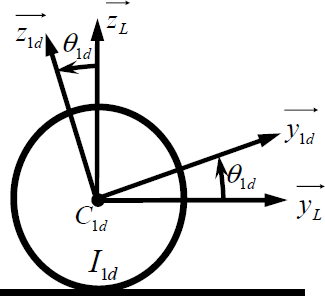
\includegraphics[width=\linewidth]{images/fig_03}

%\textit{Modèle volumique 3D}
\end{center}

\subparagraph{}\textit{À partir de la courbe précédente, analyser les performances du système de freinage électrique, sans
commande adaptée, et les comparer à celles du cahier des charges.}
\ifprof
\begin{corrige}
\end{corrige}
\else
\fi

Pour le véhicule étudié et pour la phase de freinage nominale, la composante verticale de la résultante de
l’action du sol sur l’ensemble des deux roues avant s’exprime sous la forme $F_{AV} = M(-0,26\gamma_n + 0,48g)$, avec $g$ la constante gravitationnelle. Le facteur d’adhérence au contact des pneumatiques avec le sol est d’environ 0,9.

\subparagraph{}\textit{Vérifier que le véhicule peut s’arrêter sans glisser lors d’un freinage nominal.}
\ifprof
\begin{corrige}
\end{corrige}
\else
\fi

On peut montrer que le cahier des charges impose une décélération du véhicule $\gamma(t) = \gamma_u = -\SI{6,43}{m.s^{-2}}$ en freinage d’urgence.

\subparagraph{}\textit{Vérifier que le véhicule ne peut pas s’arrêter sans glisser lors d’un freinage d’urgence.}
\ifprof
\begin{corrige}
\end{corrige}
\else
\fi

Conclusion : le système de freinage électrique doit être complété par une commande adaptée et par des freins
à disque sur les quatre roues afin de satisfaire les exigences du cahier des charges.

Remarque : il n’est pas possible de se dispenser des freins à disque pour deux autres raisons : la première est
que la batterie peut être pleine ; la deuxième est qu’à bas régime la capacité de freinage de la machine électrique
est insuffisante.
\ifprof
%\end{multicols}
\else
\end{multicols}
\fi


\end{document}

\subparagraph{}\textit{}
\ifprof
\begin{corrige}
\end{corrige}
\else
\fi

\begin{center}
\includegraphics[width=\linewidth]{images/img_04}
%\textit{}
\end{center}

